\documentclass[12pt,a4paper]{article}
\usepackage[utf8]{inputenc}
\usepackage{amsmath,enumitem,amsfonts,amssymb,graphicx,commath}
\usepackage[width=18.00cm, height=25.00cm]{geometry}
\usepackage{sectsty}
\graphicspath{ {./img/} }

\sectionfont
{\fontsize{14.4}{12}\selectfont}
\title{\textbf{Principles of AI Planning
		\\{\Large Exercise Sheet 7}}}
\makeatletter
\renewcommand{\@maketitle}
{
	\newpage
	\null
	\vskip 2em%
	\begin{center}%
		{\LARGE \@title \\ \par}%
	\end{center}%
	\par
} \makeatother

\begin{document}
\begin{flushleft}
	Authors:\\
	Erick Rosete Beas | er165@uni-freiburg.de\\
	Jessica Lizeth Borja Diaz | jb986@uni-freiburg.de\\
\end{flushleft}
{\let\newpage\relax\maketitle}
\begin{center} 
	\large 13.12.2019 
\end{center}


\section*{Exercise 8.1 - Relaxed planning graph and heuristics}

\textbf{Consider the relaxed planning task $\Pi^+$ with variables 
$A=\{a,b,c,d,e\}$, operators $O=\{o_1,o_2,o_3\}$, $o_1=\langle d, c \land (c \triangleright e)\rangle$,
$o_2= \langle c , a \rangle$, $o_3= \langle a, b\rangle$, goal
$\gamma = b \land e$ and initial states $s=\{ a\mapsto 0, 
b\mapsto 0, c \mapsto 0, d \mapsto 1, e \mapsto 0 \}$. Solve the following
by drawing the relaxed planning graph for the lowest depth $k$
that is necessary to extract a solution}
\begin{center}
	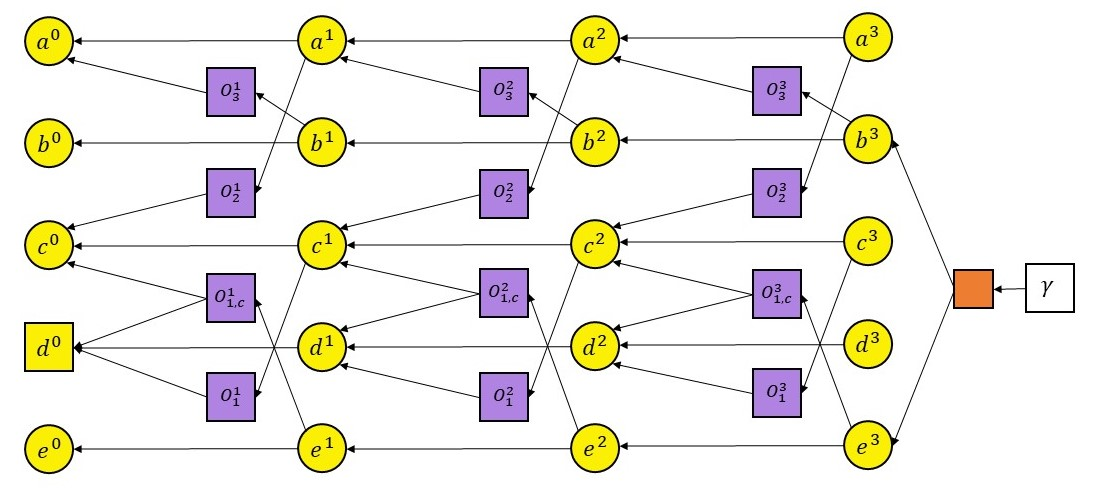
\includegraphics[scale=0.5]{img1.jpg}\\
\end{center}
\begin{enumerate}[label=(\alph*), listparindent=1.5em]
	\item \textbf{Calculate $h_{sa}(s)$ for $\Pi^+ $}\\
	The heuristic value for the initial state is 4.
	\begin{center}
		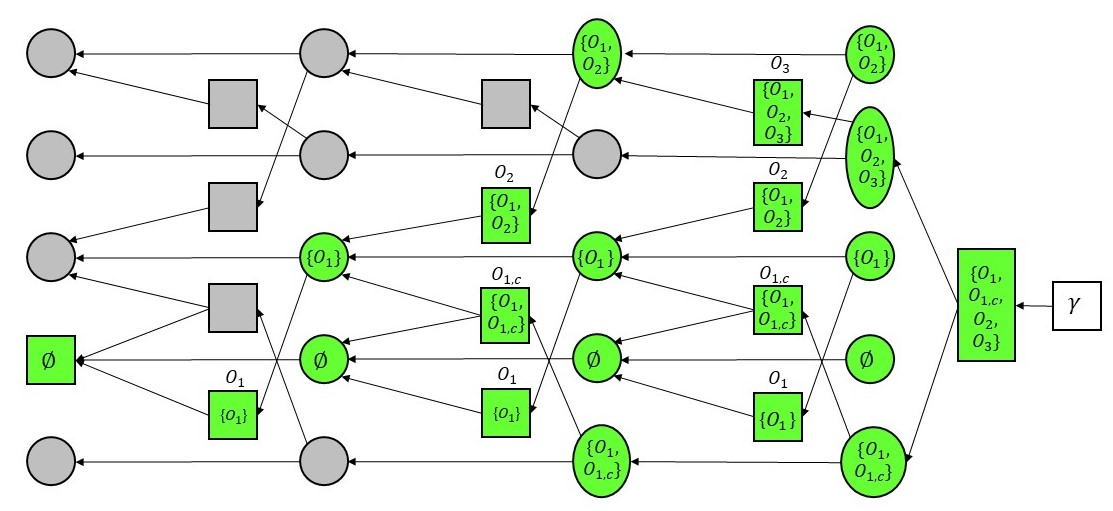
\includegraphics[scale=0.5]{hsa.jpg}\\
	\end{center}
	\item \textbf{Calculate $h_{FF}(s)$ for $\Pi^+ $}\\
	The heuristic value for the initial state is 4.
	\begin{center}
		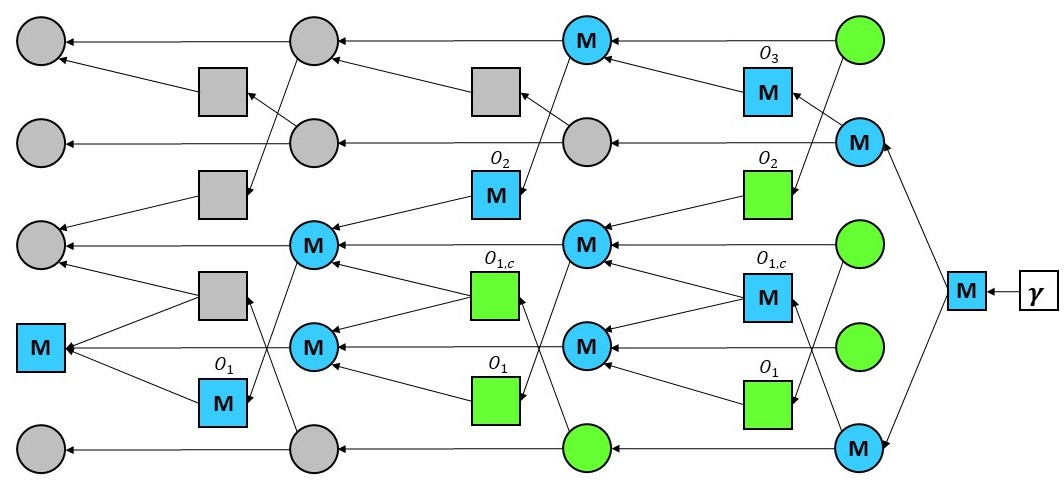
\includegraphics[scale=0.5]{hff.jpg}\\
	\end{center}
\end{enumerate}

%%%%%%%%%%%%%%%%%%%%%  Ejercicio 2 %%%%%%%%%%%%%%%%%%%%%%%%%
\section*{Exercise 8.1 - Finite domain representation}

\end{document}